% !TeX root = ../dissertation.tex
\chapter{Evaluation}

There are three main criteria by which the work is evaluated: correctness of implementation,
completeness of support for the OCaml language and runtime performance.

\section{Correctness and completeness}

Both correctness and completeness are verified by automatic testing. There are three main methods
used for this:

\begin{itemize}
      \item Trace comparison as described in Section \ref{trace-comparison}
      \item The large existing OCaml compiler test suite
      \item Automated Rust tests of components using \texttt{cargo test}
\end{itemize}

Trace comparison guarantees the behaviour is observably identical to the existing interpreter. The
OCaml test suite tests a large body of edge cases ensuring correctness and completeness.

\subsection{Initial compiler}

The initial compiler fully covers the entire bytecode instruction set. The only features not
supported are the debugger and backtraces. Implementing support for both of these features is
feasible with some work but I did not consider them important enough to spend the time to get them
working.

The compiler passes every test in the OCaml test suite except those that test backtrace
functionality. The test suite is large and extensive, having accumulated many tests over OCaml's
25year history.

The OCaml compiler is capable of bootstrapping itself from saved bytecode sources
of a previous version of the compiler with the JIT enabled. The OCaml toplevel REPL works
correctly allowing for interactive use of the JIT.

\subsection{Optimising compiler} \label{eval-opt-comp-qual}

\subsubsection{Completeness}

The optimising compiler has a slightly weaker completeness guarantee. Not all features are
supported
but those that are work correctly. The limitations are that compiler does not built handle
functions which take more than 5 arguments and the compiled functions cannot contain exception
handlers (try-catch statements) although they can raise exceptions.

The compiler gracefully fails in these cases and falls back to using the existing machine code
emitted by the initial compiler. For this reason, although the optimising compiler is not complete
in isolation the combination of the two compilers retains most of the completeness. The one
additional restriction is any dynamic libraries containing primitives using OCaml's C FFI must be
compiled to use base pointers so that the stack-walking (as described in Section \ref{gc-support})
works.

\subsubsection{Corectness}

Correctness is tested both by the OCaml compiler test suite and using a variant of the trace
comparison system comparing function parameters, return values and parameters and results of calls
to C primitives.

Correctness is mostly maintained from the original compiler with one exception: as the C/machine
stack is used rather than the OCaml stack, highly recursive functions operating on large inputs can
cause a stack overflow. This is because the OCaml stack will resize itself to larger sizes if it
fills up and because the frames on the OCaml stack are smaller.  However, this limitation does not
apply to tail-recursive functions which means that this problem is rare.

Nevertheless, this issue did cause a small number test cases to segfault on stack overflow and
represents a small regression in number of passing tests from those supported by the initial
compiler.

\section{The benchmark suite - Sandmark}

As a large part of the motivation of the project is increased performance, a core goal was to
create or integrate a suite of performance benchmarks. To do this I adapted an existing suite
called Sandmark. It is created by OCaml labs at Cambridge for their work on
multicore OCaml. It uses the \texttt{dune} build tool and the OPAM package manager to compile and
execute benchmarks.
Although the nature of the multicore OCaml project means many benchmarks were parallel, the project
also includes many sequential benchmarks with the purpose of ensuring the work on the multicore
runtime does not create single core performance regressions.

It took a some effort to adapt the suite to work for my purposes. The existing suite was only
supported native code programs so it had to be adapted to work with bytecode instead. Now running
all the benchmarks and collating the results only requires executing a single script.

\subsection{Selection of programs}

The suite includes hundreds of benchmarks with support for tweaking benchmark parameters increasing
this even more. In order to keep full execution time to about 3 hours, I settled on a suite of 36
programs taken from Sandmark's \texttt{macro} subcategory. These programs used many different
language features with different workloads. Some were numeric (both integer and floating point),
some tested asynchronous behaviour with \texttt{Lwt} and others tested use of OCaml libraries like
the \texttt{yojson} JSON parser.

\section{Benchmark results}

Four different configurations of the OCaml runtime are described in this section:

\begin{enumerate}
      \item The stock OCaml 4.11.1 bytecode interpreter without any modifications
      \item The state of the JIT after creating the initial compiler (the `old' initial compiler)
      \item The current state of JIT with the optimising compiler disabled, but retaining
            the modifications made to the initial compiler to support dynamic recompilation (the
            `current' initial compiler)
      \item The full current JIT including the optimising compiler with the hot function threshold
            set to 50 (the optimised compiler)
\end{enumerate}

In order to allow for easier comparison between programs, I am comparing all JIT results relative
to the baseline of the stock bytecode interpreter to obtain relative speedup values; these are
calculated by
dividing the stock interpreter time by the corresponding JIT time.

\subsection{Overview}

\begin{figure}[h]
      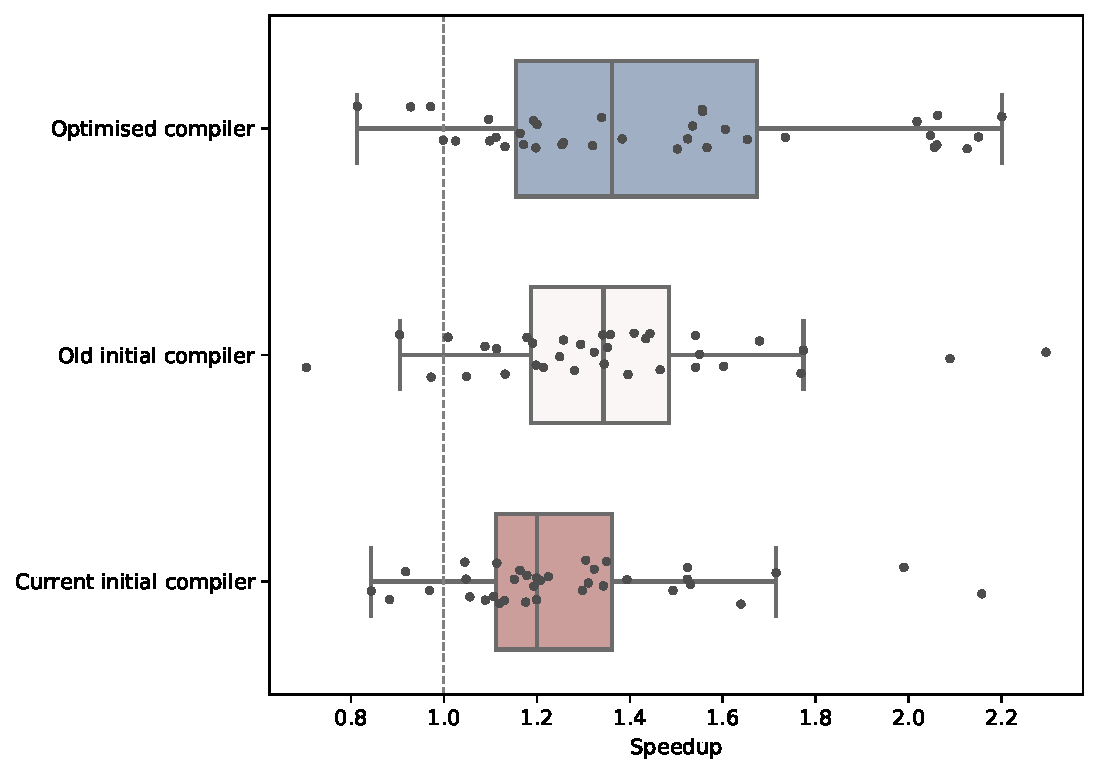
\includegraphics[width=\textwidth]{box}
      \caption{Distribution of speedup values for each version of the JIT}
      \label{fig:box}
\end{figure}

Figure \ref{fig:box} shows the high level summary of results on the execution speedup time. The
chart shows a standard box plot
\footnote{Lines for minimum, lower quartile, median, upper quartile and maximum. Outliers (outside
      1.5 of the interquartile range) are not included in the whiskers}
with points for each result overlaid. The points are vertically
offset randomly.

The general trend is of an increased execution time for most programs on all 3 compilers. The
initial compiler as it existed before the changes made in section \ref{dyn-recomp} was faster than
the current version.

The combination of the optimised compiler and current initial compiler version performed slightly
worse on programs in the lower half of the speed distribution  which can be seen by the decreased
lower quartile value.  However it had a slightly increased median and much better on the top half
of the distribution with a cluster of 8 programs managing to half the execution time relative to
the stock interpreter.

Although most programs tested benefited from the changes, about 4 programs did not and had
decreased performance.

\subsection{Analysis}

In order to understand these trends and investigate anomalies it is useful to show the results for
each individual benchmark program. Figure \ref{fig:perf} shows the relative speedup values for each
benchmark program, ordered by decreasing optimising compiler speedup.

We notice that there are a few different patterns:

\begin{itemize}
      \item In some programs for which the improvements were roughly equivalent for all types of
            program
            such as \texttt{chameneos\_redux\_lwt}.
      \item In some the optimising compiler addded significant performance gains such as
            \texttt{revcomp2} and \texttt{pidigits5}.
      \item In nearly all cases the new version of the initial compiler was slower than the initial
            version.
      \item In most cases the optimising compiler increased performance above the initial compiler
            alone.
\end{itemize}

In order to explain these patterns it is necessary to consider the cost and potential benefits of
each version of the compiler:

\subsubsection{Initial version of initial compiler}

The main change from the bytecode is replacing the interpreter with machine code performing the
same
operations but with the operations inlined into their uses. The main cost of this is an increased
pressure on the instruction cache. However, this also allows for the CPU to more effectively
predict
the sequence of execution allowing for less pipeline hazards, better branch prediction and
out-of-order execution across bytecode boundaries.

For most programs this trade-off is worth it.  The programs where it isn't (\texttt{fft},
\texttt{nbody} and \texttt{durand-kerner-arberth}) all show heavy use of floating point operations
meaning most of the work is done using C primitives and boxed floats. This means most of the time
spent executing these programs is in allocating and freeing boxed floats from the heap within the C
primitives implementing floating point operations.

\subsubsection{Current version of initial compiler}

The main significant change in this version was the extra level of pointer indirection on closure
code fields requiring one more memory load to call a closure. For this reason, in nearly all cases
this represented a slowdown from the initial compiler. The differing amounts of slowdown reflects
the variation in benchmark hot path behaviour. Where it is a large drop, it reflects programs with
large number of calls to shorter programs and where it is small it indicates larger functions
making less calls or spending much of their time in C primitives.

\begin{landscape}
      \begin{figure}[h]
            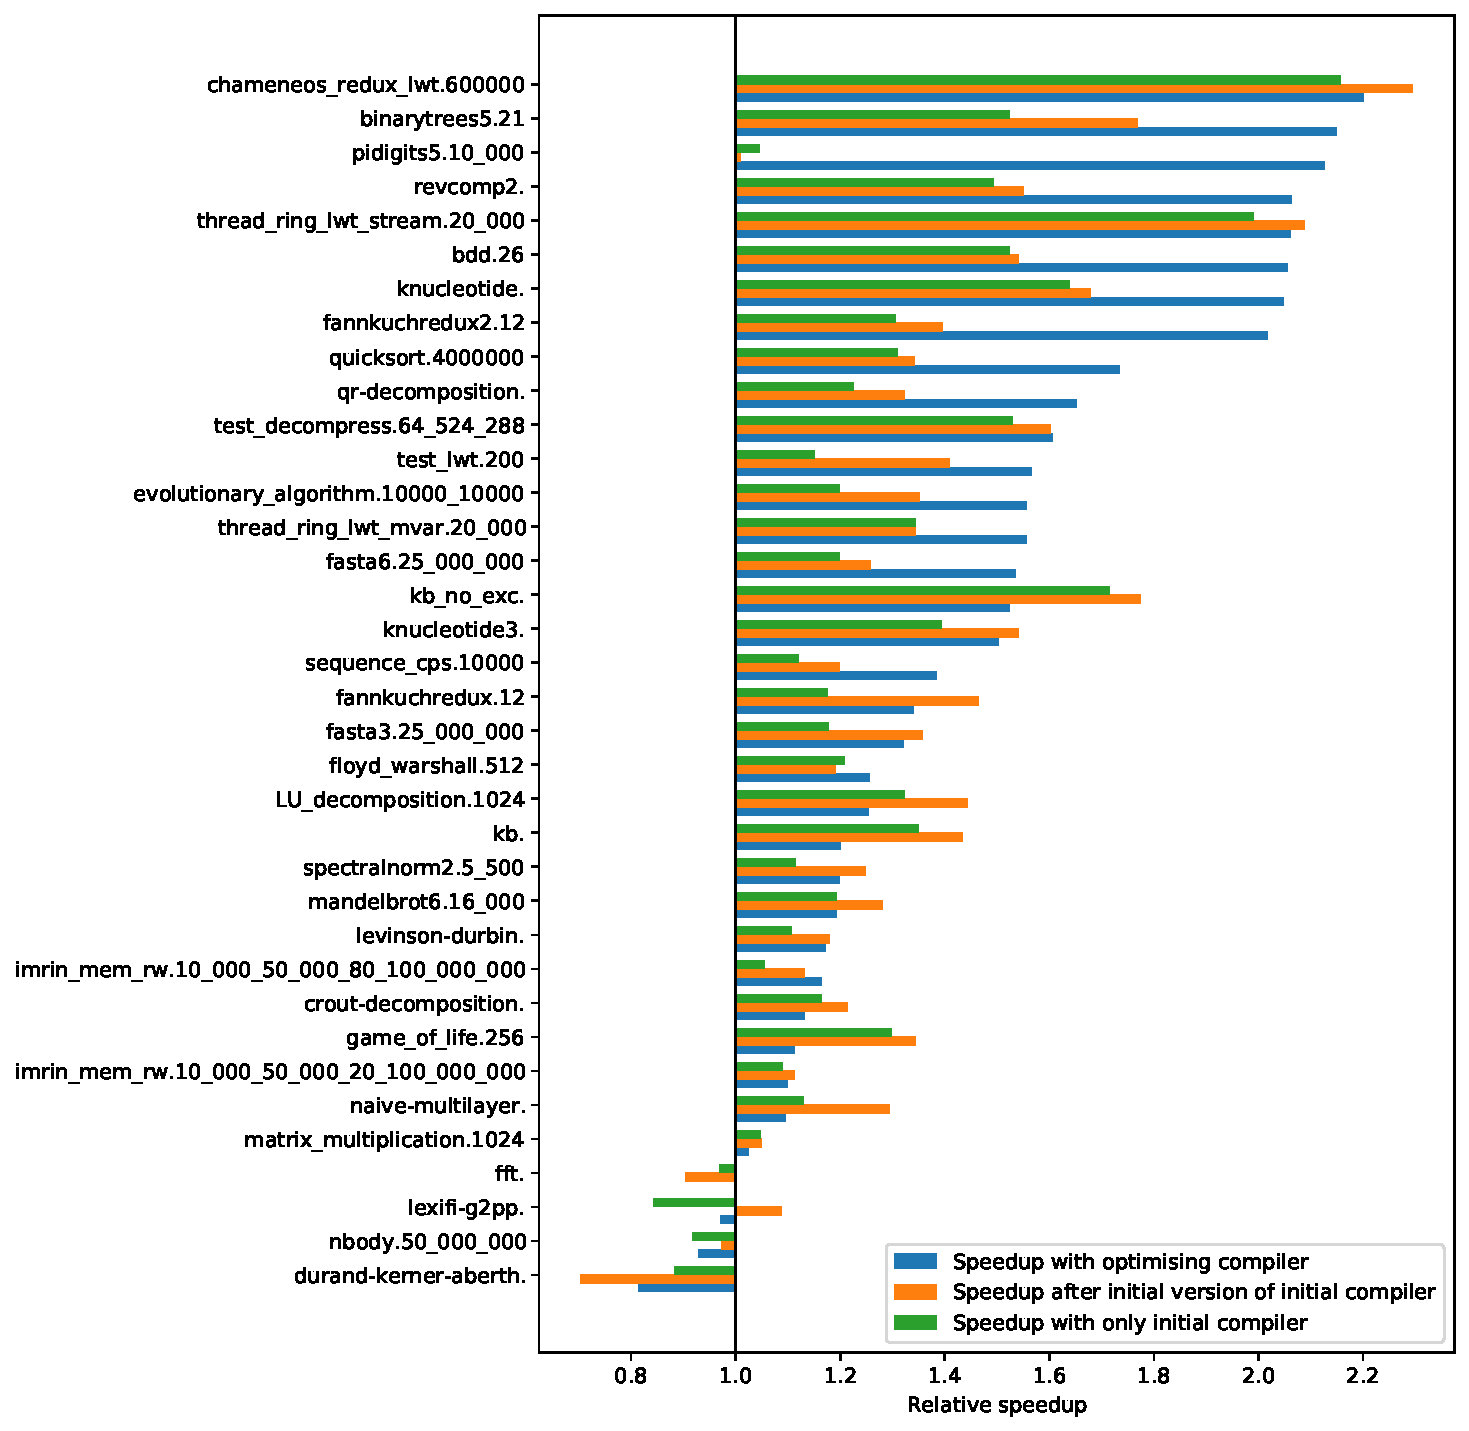
\includegraphics{perf}
            \caption{Speedup values for each benchmark}
            \label{fig:perf}
      \end{figure}
\end{landscape}

\subsubsection{Optimising compiler}

The optimising compiler has a more significant compilation cost. However, this is easily amortised
over the long running time of the benchmark programs (see \ref{bias-exec-time}). The major change
from the other two methods and the interpreter is the use of registers rather than the OCaml stack
for storing intermediate values.

In most cases this led to better performance than current version of the initial compiler
suggesting
that the optimising compiler's code is generally faster. Where it isn't, it would suggest that the
overhead of switching back and forth between using registers for arguments and the OCaml stack as
happens at the boundary between optimised and unoptimised functions is overwhelming any performance
benefits.

We would expect the most significant gains where a chain of multiple optimised functions can call
each-other in turn: this is the pattern shown by many of the cases where the optimising exceeds the
performance of the old version of the initial compilers. A case where this is particularly obvious
is in
\texttt{pidigits} where the optimising compiler was twice as fast as both initial compiler only
runs
(which themselves ran at about the same speed as the stock interpreter).

In half of the cases where the optimising compiler compiler is faster than the current initial
compiler, it is able to overcome the overhead imposed by the extra pointer lookup on function
calls; in many
case significantly slow.

In the other half of cases, performance for the optimising compiler is comparable but slightly
worse
than the new initial compiler.

One case causing this is demonstrated in \texttt{mandlebrot6} - here the main loop is implemented
in
imperative style at the root level of the module using a while loop rather than recursion. This
means that the optimising compiler will never attempt to optimise it. It additionally makes use of
exceptions which are not well supported by the optimising compiler (see Section
\ref{exception-handling}).

\section{Bias}

Although Sandmark is more representative of real OCaml workloads than many benchmark suites there
are some biases:

\subsubsection{Execution time} \label{bias-exec-time}

Execution times ranged from \SI{1}{\second} to \SI{500}{\second}. Of the 36 benchmarks, 13 took
below \SI{10}{\second} and 7 took above \SI{50}{\second}.  In the context of this project, this
means all programs classify as somewhat long-running and time spent on compilation was a negligible
factor - my manual testing estimates this overhead to be the order of magnitude of at most
\SI{300}{\nano\second} for JIT-compiling the entire OCaml compiler, which is a particularly large
OCaml program.

\subsubsection{Work done}

Nearly all of the benchmarks included the same work being done many times in a hot loop. This is
the best case for modern CPUs and dynamically optimising compilers.

Although the performance of programs is dominated by the hot path loops, larger programs tend to
also have more cold code executed once or only a few times. This is less well tested.

\section{Summary}

The initial compiler increased performance for most tested programs while retaining the semantics
and the ability to run all OCaml bytecode programs.

Adding the optimised compiler led to significantly increased execution time on some tested programs
while decreasing the time for others. Across the suite of benchmark programs it caused large
improvement in half of programs and slightly decrease in the other half; overall it was an
improvement.

All of this was achieved while retaining support for all OCaml features without compromising
correctness.